\chapter{\MakeUppercase{Introdução}}
\label{chap:intro}
\thispagestyle{plain}

\vspace{-3em} % Ajusta o valor para reduzir o espaçamento

O problema de segurança pública sempre foi um problema no Brasil. Constantes crimes de furtos e roubos geram grandes danos, principalmente financeiros, tanto para o indivíduo, no caso das vítimas, quanto para a sociedade \cite{Cerqueira2007, G12013}. Um dos reflexos gerados por essa insegurança está no fato de que vários locais públicos devem ter seu acesso controlado e vigiado para garantir a segurança patrimonial.

As \textit{smart cities} (cidades inteligentes) estão emergindo como uma prioridade para pesquisa e desenvolvimento em todo o mundo. Elas abrem oportunidades significativas em várias áreas, como crescimento econômico, saúde, bem-estar, eficiência energética e transporte, para promover o desenvolvimento sustentável das cidades \cite{Song2017}. O conceito e oportunidades das \textit{smart cities} são escaláveis para outros conceitos ‘smart’ como o \textit{smart room}, \textit{smart home}, \textit{smart building}, etc \cite{Pacheco2018}. A proliferação de tecnologias de informação e comunicação possibilita o desenvolvimento de diversos serviços inteligentes. E um dos serviços comunitários mais essenciais é justamente a vigilância inteligente \cite{Chen2016, Nikouei2018}.

Nos últimos anos, aplicações de reconhecimento facial a partir de imagens geradas por câmeras de videomonitoramento têm ganhado relevância, sendo largamente utilizadas para a verificação ou identificação de indivíduos em locais públicos. No âmbito da segurança, o reconhecimento facial em vídeo permite agilidade nas situações em que muitos indivíduos devem ser identificados rapidamente \cite{Quirita2014}.

Apesar de estarmos longe de conseguir com que a IA (inteligência artificial) se aproxime da performance humana, em algumas áreas, como reconhecimento de imagem, carros autônomos e jogos eletrônicos, ela se mostra equivalente, ou até mesmo superior \cite{Aggarwal2018}. Em tarefas de visão computacional é possível rastrear o movimento de uma pessoa em um plano de fundo complexo. E com moderado sucesso, é possível tentar localizar e nomear todas as pessoas em uma fotografia, através da detecção e reconhecimento de faces, roupas e cabelos \cite{Szeliski2011}.

O \textit{deep learning} (aprendizagem profunda), ramo do \textit{machine learning} (aprendizagem de máquina), tornou-se imensamente popular no reconhecimento de imagens, bem como em outras tarefas de reconhecimento e correspondência de padrões \cite{Verhelst2017}.

As redes neurais artificiais simulam o sistema nervoso humano com base em aprendizado de máquina, tratando as unidades computacionais em um modelo de aprendizado de maneira semelhante aos neurônios humanos. Não é uma tarefa fácil pois o poder computacional do computador mais rápido atualmente equivale a uma pequena fração do poder computacional de um cérebro humano \cite{Aggarwal2018}.

As \textit{deep neural networks} (redes neurais profundas) envolvem uma complexidade computacional significativa, fazendo com que, até recentemente, seu processamento fosse viável apenas em plataformas de potentes servidores disponíveis na ‘nuvem’ \cite{Verhelst2017}. Quando é necessário armazenamento e computação de dados em larga escala, a computação em nuvem tem sido a solução. Porém, com o grande crescimento de dispositivos móveis e inteligentes, juntamente com as tecnologia de IoT (Internet das Coisas), o foco mudou para se obter respostas em tempo real. \cite{Dolui2017}.

Nos últimos anos, vê-se uma tendência de se incorporar o processamento de aprendizado profundo em dispositivos de borda, como celulares, dispositivos móveis e nos nós da IoT. Isso torna possível a análise de dados localmente, em tempo real, além de mitigar problemas de privacidade dos dados \cite{Verhelst2017}. Outro benefício da computação na borda (\textit{Edge Computing}) é o descongestionamento da rede de dados, pois permite que o processamento seja feito próximo das fontes dos dados \cite{Merenda2020}. Assim, evita-se a comunicação desnecessária, que sobrecarrega não só a rede principal como também o datacenter na nuvem \cite{Aazam2014}.

No contexto de um sistema de monitoramento inteligente de vários ambientes, com reconhecimento facial, representado na figura \ref{fig:sistemCentralizado}, várias câmeras capturam imagens de maneira constante e simultânea. Essas imagens precisam ser enviadas de forma integral para um servidor central responsável pelo processamento, incluindo a detecção e reconhecimento de faces. Nesse paradigma, surgem desafios significativos, como o elevado volume de dados que sobrecarrega a rede, a possível degradação do tempo de resposta devido à concorrência no processamento centralizado e a dificuldade inerente à escalabilidade do sistema, entre outros.

\begin{figure}[H]
    \centering
    \caption[Arquitetura de processamento centralizado, onde as imagens capturadas pelas câmeras são enviadas integralmente para uma unidade central de processamento.]{Arquitetura de processamento centralizado, onde as imagens capturadas pelas câmeras são enviadas integralmente para uma unidade central de processamento}
    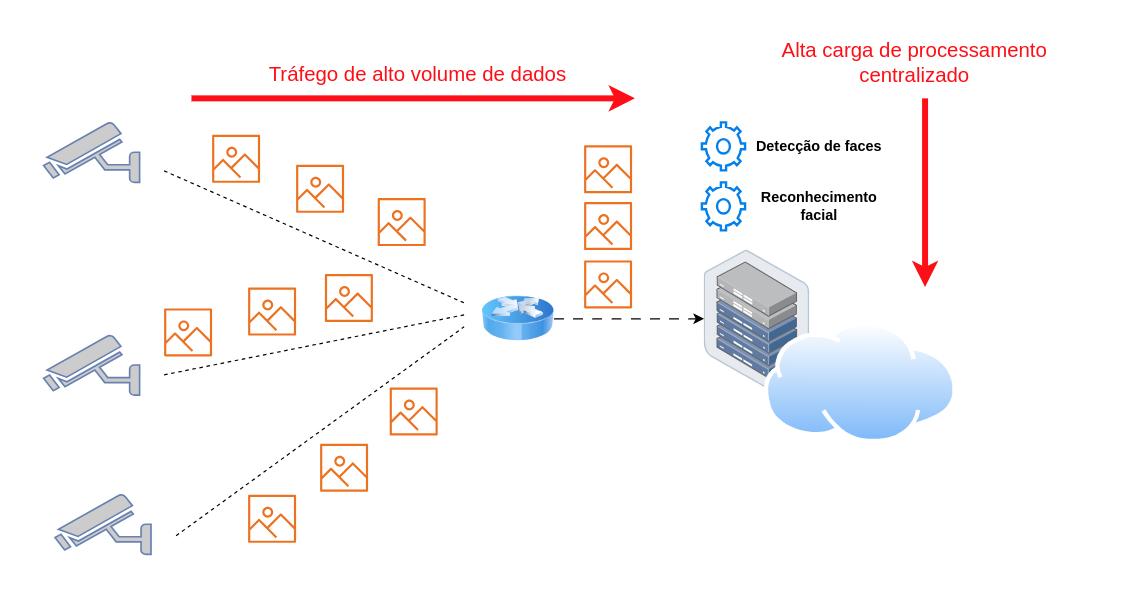
\includegraphics[width=0.9\textwidth]{Cap1_Introducao/Figures/sistema_centralizado.png}
    \caption*{Fonte: autor.}
    \label{fig:sistemCentralizado}
\end{figure}

Ao adotar o paradigma de processamento distribuído, surge uma solução promissora para os desafios mencionados, oferecendo a possibilidade de descentralizar parte do processamento. A utilização de dispositivos SBCs permite trazer parte do processamento, como o processo de detecção facial, para a borda, enquanto o reconhecimento facial permanece centralizado, como representado pela figura \ref{fig:sistemDistribuido}. Essa abordagem não apenas alivia a carga nos servidores centrais, mas também reduz significativamente o tráfego de dados pela rede, uma vez que apenas as imagens das faces identificadas precisam ser encaminhadas para os servidores centrais para as demais etapas de processamento. Além disso, essa arquitetura distribuída proporciona uma escalabilidade mais eficiente, permitindo a adição de novos pontos de monitoramento de forma simplificada, sem comprometer o desempenho do sistema como um todo.

\begin{figure}[H]
    \centering
    \caption[Arquitetura de processamento distribuído, onde a detecção de faces ocorre na borda, enquanto o reconhecimento facial permanece centralizado.]{Arquitetura de processamento distribuído, onde a detecção de faces ocorre na borda, enquanto o reconhecimento facial permanece centralizado.}
    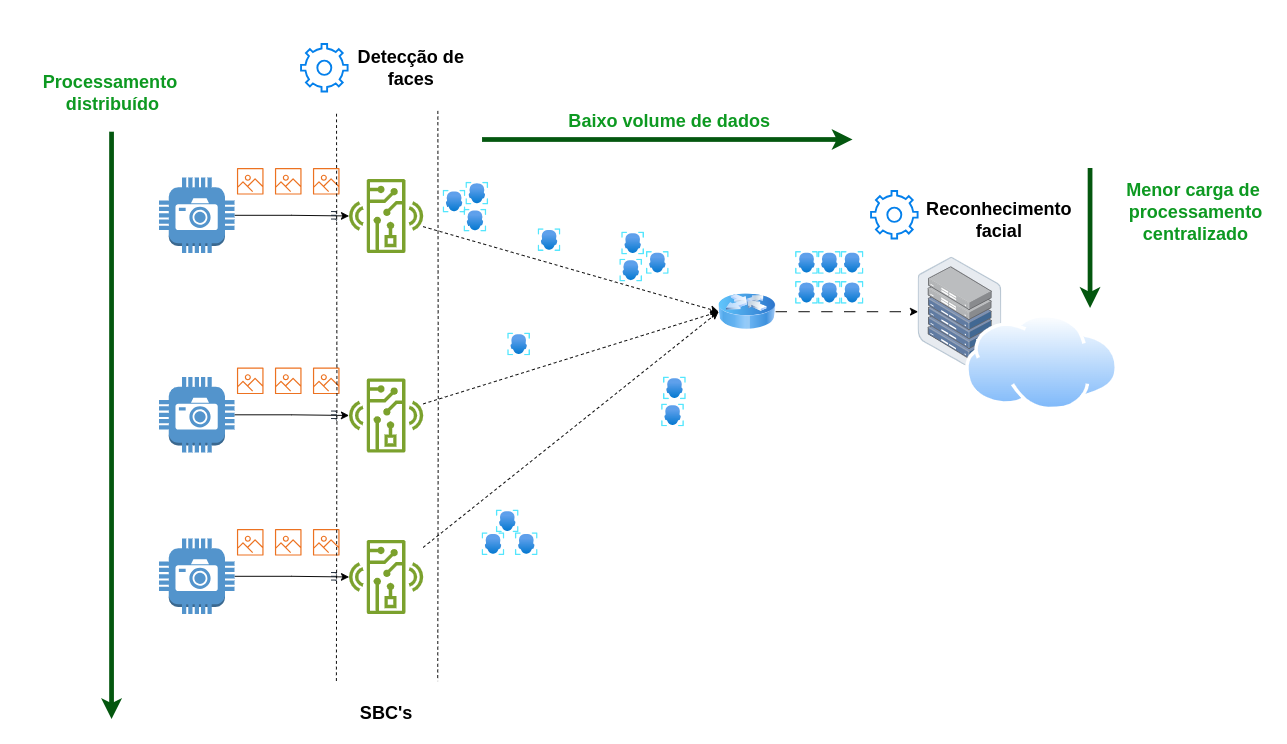
\includegraphics[width=0.9\textwidth]{Cap1_Introducao/Figures/sistema_distribudo.png}
    \caption*{Fonte: autor.}
    \label{fig:sistemDistribuido}
\end{figure}

\section{Objetivo Geral}

Com este trabalho objetiva-se testar o desempenho de dispositivos de borda no processo de detecção de faces, avaliando sua capacidade de detecção e tempo de resposta para diferentes cenários, com possíveis aplicações de monitoramento inteligente e controle de acesso. Com os resultados obtidos, espera-se determinar, para cada cenário definido, se o dispositivo é capaz de processar de forma satisfatória a etapa de detecção de faces, e as vantagens de se realizar esse processo na borda, em uma arquitetura de processamento distribuído.

\subsection{Objetivos Específicos}
Em um sentido mais estrito, pretende-se
\begin{itemize}
    \item Definir diferentes cenários (com aplicabilidade para monitoramento inteligente e controle de acesso) e os requisitos a serem cumpridos, como tempos de respostas e capacidade de detecção de faces. Serão utilizadas imagens estáticas que representem cada cenário para os testes.
    \item Desenvolver um sistema para auxiliar na parametrização do algoritmo de detecção, buscando melhor otimização para cada cena e dispositivo, e na obtenção das métricas de desempenho.
    \item Analisar os resultados obtidos e determinar para quais cenários os dispositivos podem executar a detecção de face de forma satisfatória e quais os ganhos em se executar tal processamento na borda, principalmente no que se refere à utilização de banda na rede de um sistema com arquitetura de processamento distribuído, sua escalabilidade e tempos de resposta.
\end{itemize}

\section{Estrutura do Texto}
O texto desse trabalho foi dividido em cinco capítulos. No Capítulo 1, Introdução, é feita uma contextualização do cenário no qual o tema de pesquisa desse trabalho está inserido, além de tratar dos objetivos geral e específicos. No Capítulo 2, Revisão Teórica, é feita uma explanação sobre os conceitos e técnicas existentes que servem como embasamento para o que foi proposto e desenvolvido. No capítulo 3, Desenvolvimento, são apresentadas as etapas, técnicas e ferramentas utilizadas para a realização dos experimentos e obtenção dos resultados. No Capítulo 4, Experimentos Realizados, são apresentados todos os passos realizados na experimentação, os dados obtidos, bem como as análises e algumas conclusões. E, por fim, no Capítulo 5, como o próprio título diz, são feitas as considerações finais e possíveis trabalhos futuros são abordados.
